\documentclass[12pt]{article}
\usepackage{fullpage}
\usepackage{epsf}
\usepackage{graphicx}
\usepackage{listings}
\lstset{
   breaklines=true,
   basicstyle=\ttfamily}

\newtheorem{definition}{Definition}
\newtheorem{property}{Property}
\newtheorem{proof}{\em Proof}
\newtheorem{derivation}{\em Sketch}
\newtheorem{notation}{Notation}

\newcommand{\comment}[1]{}
\newcommand{\VS}{\mbox{\it VS}}
\newcommand{\WM}{\mbox{\it WM}}
\newcommand{\PCONJ}{\mbox{\it PCONJ}}
\newcommand{\kDNF}{\mbox{\it kDNF}}
\newcommand{\PDISJ}{\mbox{\it PDISJ}}
\newcommand{\DTrt}{\mbox{\it DT}_{r2}}
\newcommand{\DTs}{\mbox{\it DT}_s}
\newcommand{\PP}{{\rm P}}
\newcommand{\EE}{{\rm E}}
\newcommand{\PX}{\PP_{\!\scriptscriptstyle\! X}}
\newcommand{\PXY}{\PP_{\!\scriptscriptstyle\! X\!Y}}
\newcommand{\PYX}{\PP_{\!\scriptscriptstyle\! Y\!|\!X}}
\newcommand{\PYx}{\PP_{\!\scriptscriptstyle\! Y\!|x}}
\newcommand{\seq}[1]{\langle{#1}\rangle}
\newcommand{\RR}{I\!\!R}
\newcommand{\NN}{I\!\!N}
\newcommand{\argmin}{\arg\!\min}
\newcommand{\argmax}{\arg\!\max}
\newcommand{\eg}{{\em e.g.},\ }
\newcommand{\Eg}{{\em E.g.},\ }
\newcommand{\ie}{{\em i.e.},\ }
\newcommand{\Ie}{{\em I.e.},\ }
\newcommand{\cf}{{\em cf.}\ }
\newcommand{\etc}{{\em etc}}
\newcommand{\aka}{{\em a.k.a.}}
\newcommand{\vardef}{\stackrel{\triangle}{=}}
\def\norm [#1]{{\| #1 \|}}
\newcommand{\sign}{\mbox{\rm sign}}
\newcommand{\err}{\mbox{\rm err}}
\newcommand{\rank}{\mbox{\rm rank}}
\newcommand{\cond}{\mbox{\rm cond}}
\newcommand{\vect}{\mbox{\rm vec}}
\newcommand{\tr}{\mbox{\rm tr}}
\newcommand{\set}[1]{{\{#1\}}}
\newcommand{\tnorm}[2]{\|{#1}\|_{#2}}
\newcommand{\normdot}{{\mbox{$\|\!\cdot\!\|$}}}

%\newcommand{\makevector}[1]{{\tilde{#1}}}
\newcommand{\makevector}[1]{{\bf #1}}
\newcommand{\fvec}{{\makevector{f}}}
\newcommand{\evec}{{\makevector{e}}}
\newcommand{\bvec}{{\makevector{b}}}
\newcommand{\rvec}{{\makevector{r}}}
\newcommand{\dvec}{{\makevector{d}}}
\newcommand{\xvec}{{\makevector{x}}}
\newcommand{\qvec}{{\makevector{q}}}
\newcommand{\yvec}{{\makevector{y}}}
\newcommand{\mvec}{{\makevector{m}}}
\newcommand{\vvec}{{\makevector{v}}}
\newcommand{\zvec}{{\makevector{z}}}
\newcommand{\avec}{{\makevector{a}}}
\newcommand{\wvec}{{\makevector{w}}}
\newcommand{\cvec}{{\makevector{c}}}
\newcommand{\Xvec}{{\makevector{X}}}
\newcommand{\Fvec}{{\makevector{F}}}
\newcommand{\Avec}{{\makevector{A}}}
\newcommand{\Bvec}{{\makevector{B}}}
\newcommand{\Hvec}{{\makevector{H}}}
\newcommand{\Lvec}{{\makevector{L}}}
\newcommand{\Mvec}{{\makevector{M}}}
\newcommand{\Nvec}{{\makevector{N}}}
\newcommand{\Vvec}{{\makevector{V}}}
\newcommand{\Uvec}{{\makevector{U}}}
\newcommand{\Ivec}{{\makevector{I}}}
\newcommand{\Ovec}{{\makevector{O}}}
\newcommand{\smallxvec}{{\scriptsize\mathbf x}}
\newcommand{\alphavec}{\mbox{\boldmath $\alpha$}}
\newcommand{\betavec}{\mbox{\boldmath $\beta$}}
\newcommand{\muvec}{\mbox{\boldmath $\mu$}}
\newcommand{\phivec}{{\mbox{\boldmath $\phi$}}}
\newcommand{\lambdavec}{\mbox{\boldmath $\lambda$}}
\newcommand{\Lambdavec}{\mbox{\boldmath $\Lambda$}}
\newcommand{\Sigmavec}{\mbox{\boldmath $\Sigma$}}
\newcommand{\yy}{{\tt y}}
\newcommand{\uu}{{\tt u}}
\newcommand{\zerovec}{{\makevector{0}}}
\newcommand{\smallzerovec}{{\scriptsize\bf 0}}
\newcommand{\smallonevec}{{\scriptsize\bf 1}}
\newcommand{\onevec}{{\makevector{1}}}
\newcommand{\smallbetavec}{\mbox{\scriptsize\boldmath $\beta$}}
\newcommand{\smallmuvec}{\mbox{\scriptsize\boldmath $\mu$}}


\begin{document}

\noindent
Parley Pacheco Martins 1484000\\
AUCSC 460 -- Artificial Intelligence\\
Winter 2016\\
Department of Science\\
University of Alberta, Augustana Faculty

\vspace*{0.75\baselineskip}
\hrule
\vspace*{0.75\baselineskip}

\noindent
{\Large\bf Report Rock Paper Scissors }

%%%%%%%%%%%%
\section{Game Agent}

The first dumb agent (SimpleCycleAgent) is just a simple cycle made to beat the Rock, Paper, Scissors cycle.
It doesn't react to the other agent and always play this cycle.
This agent was made just to see the behavior (of both of the agents) when such a simple one is playing.

The second agent (BiggerCycleAgent) is another dumb cycle, but bigger.
It chooses a random cycle size from 1000 to 10000 and randomly populates the cycle.
Once it's done, it just iterates through the cycle, without any reaction.
This was done to improve the challenge of finding a cycle, since this can be really tricky for other agents.
Depending on the size of the cycle it's not really different from the RandomAgent.

The third agent (StatisticAgent) is ``smarter'', in the sense that it reacts to the other player.
It counts the frequency of a movement and plays the action that would beat the most played action by the oponent.
This was actually the first idea, but I think it would have been more successful against humans, since we are horrible at ramdonness.

% \end{lstlisting}


%%%%%%%%%%%%
\section{Results}

The three agents had the following results:

\begin{figure}[h]
\caption{StatisticAgent against the others}
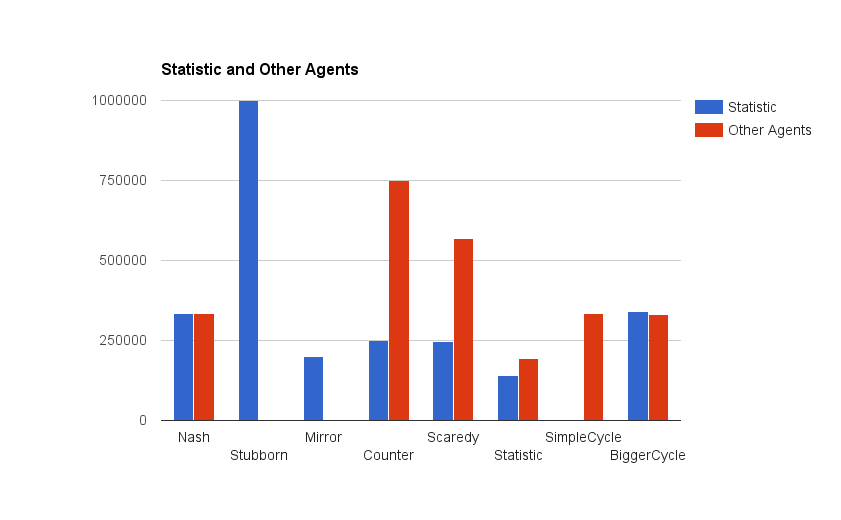
\includegraphics[width=\textwidth]{images/statistic.png}
\end{figure}

\begin{figure}[h]
\caption{SimpleCycleAgent against the others}
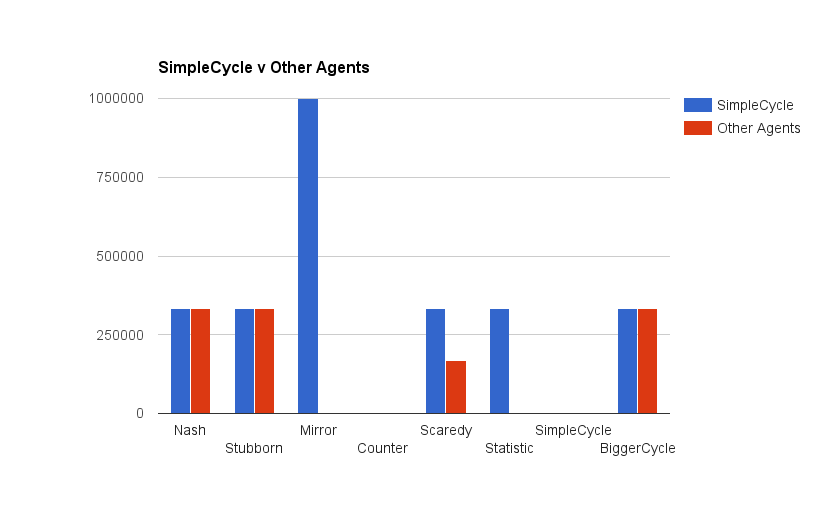
\includegraphics[width=\textwidth]{images/simple_cycle.png}
\end{figure}

\begin{figure}[h]
\caption{BiggerCycleAgent against the others}
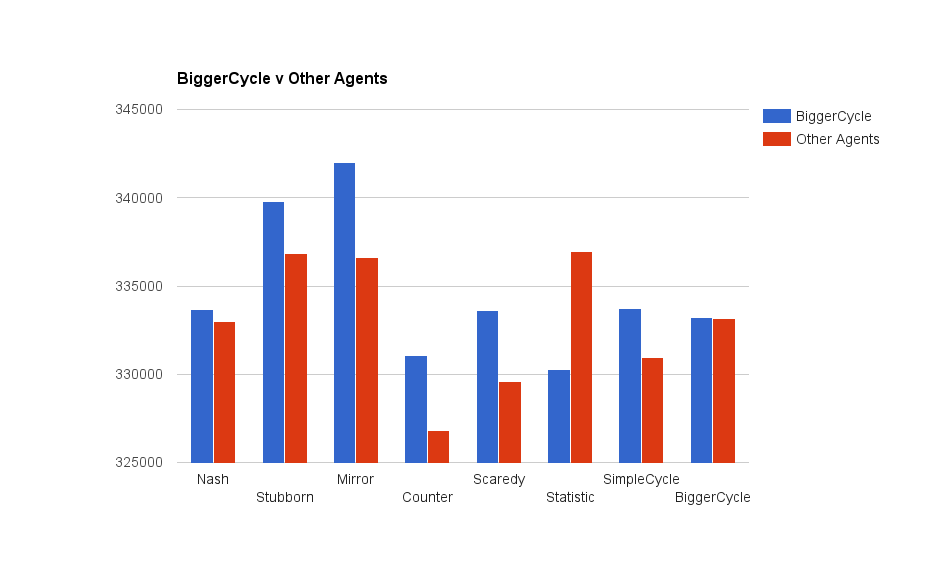
\includegraphics[width=\textwidth]{images/bigger_cycle.png}
\end{figure}
%%%%%%%%%%%%
\section{Performance Discussion}

%%%%%%%%%%%%
\section{Other Approaches}

%%%%%%%%%%%%
\section{Conclusion}

\end{document}
